\chapter{多波干涉与光栅}\label{ch:b2:gratings}

将一张光盘斜置于灯下，它便映出彩虹：其螺旋
线上的凹坑相隔 1.5 微米，本身便是一块光栅——成千上万
条微小的反射条带，每条都反射一份波，全部
相互干涉。两列波给出前几章所见的柔和 $\cos^2$ 条纹；
一千列波则给出窄千倍的条纹，锐利得
足以分辨两个波长，二者相差仅
十万分之一。这正是借以测定太阳成分的仪器，
星系的速率也由它测出，它也装在每台光谱仪中。
本章叠加 $N$ 列波，推导光栅
方程，讨论其色散与分辨本领，并介绍另一种
多波干涉装置——法布里–珀罗腔，它将成为
激光器的谐振腔。

\begin{omfigure}
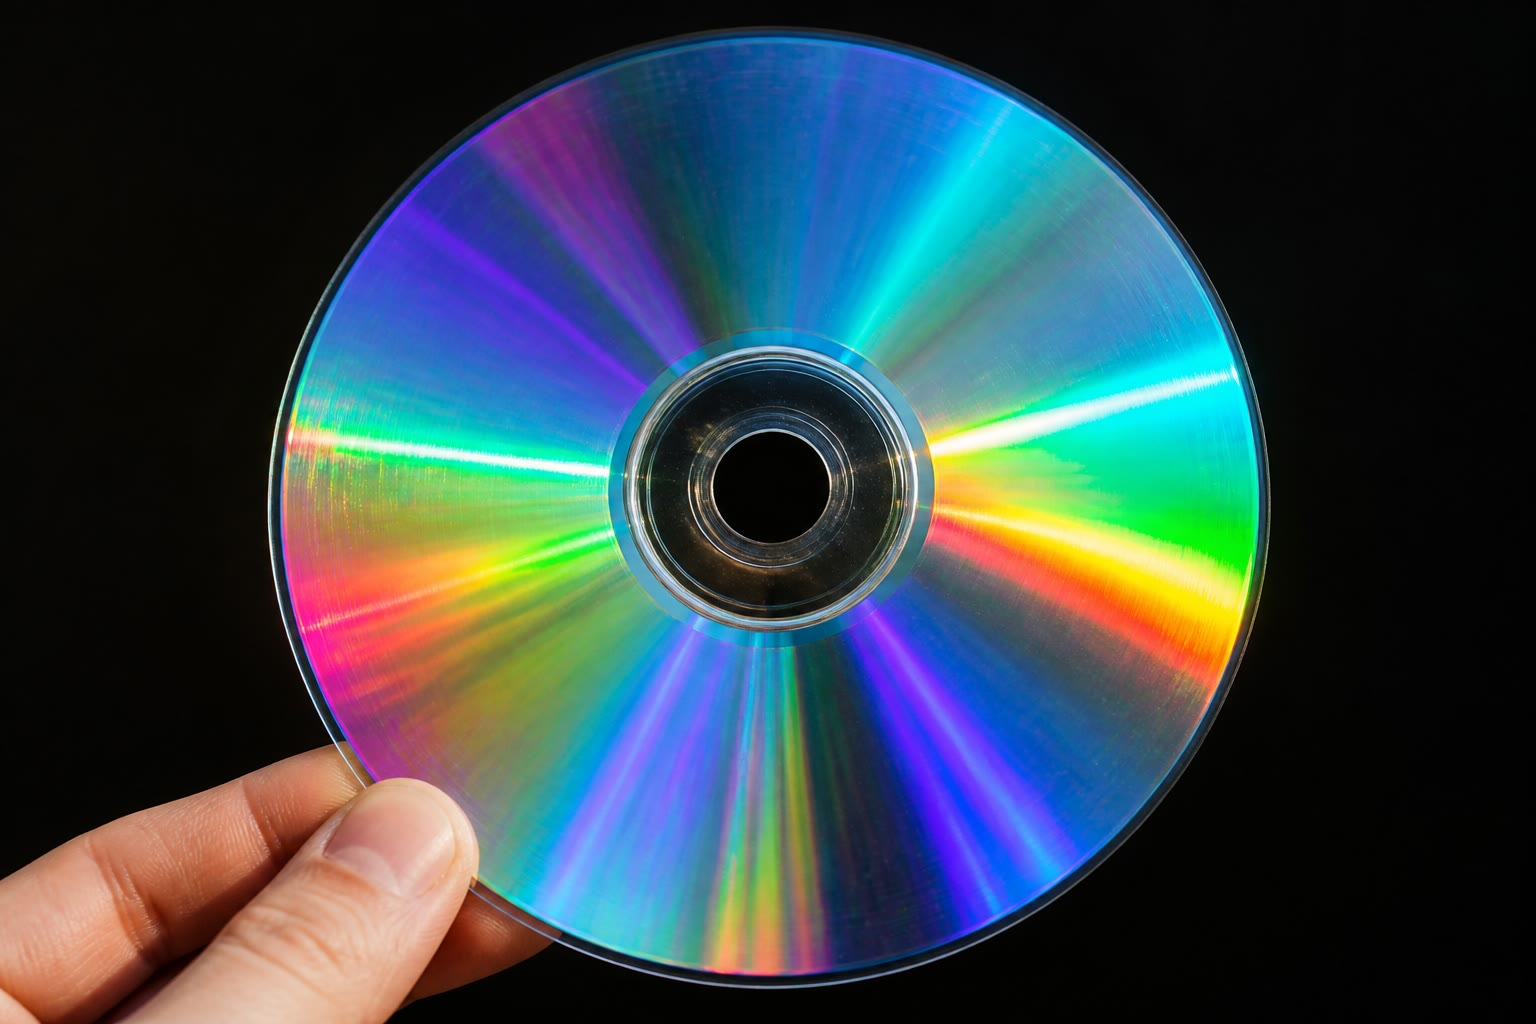
\includegraphics[width=0.54\linewidth]{images/book4/ai/b4-21-cd-diffraction-colours.jpg}

{\small 阳光下的光盘：其螺旋线上的凹坑相隔 $\qty{1.6}{\micro m}$，构成一块反射光栅，每一级衍射将白光展开为光谱。}
\end{omfigure}

\section{$N$ 列波的干涉}

\begin{theorem}[相位成等差的 $N$ 列等幅波]\label{thm:b2:gratings:nwaves}
\index{多波干涉}\index{主极大}\index{次极大}\index{相量}
$N$ 列相干的等幅波，振幅均为 $a$，各列比前一列落后
相位 $\varphi$，叠加成振幅为 $A(\varphi)$ 的波，其
强度为
\[
A = a\,\frac{\sin(N\varphi/2)}{\sin(\varphi/2)} , \qquad
I(\varphi) = I_0\,\frac{\sin^2(N\varphi/2)}{\sin^2(\varphi/2)} :
\]
\emph{主极大}的强度为 $N^2I_0$，位于 $\varphi = 2\pi p$ 处（各列波
同相），角半宽为 $2\pi/N$（按 $\varphi$ 计，第一零点
位于 $\varphi = 2\pi p \pm 2\pi/N$ 处），之间隔有 $N - 2$ 个\emph{次极大}
其高度至多约为主极大的 $4.5\%$，在
$N$ 较大时。列数越多，峰越窄越亮：宽度
按 $1/N$ 缩小，高度按 $N^2$ 增长，能量
（即二者之积）随 $N$ 增长。
\end{theorem}

\begin{proof}
复振幅为 $a\eu^{\iu k\varphi}$，$k = 0, \dots, N - 1$：一个等比
级数，$a(1 - \eu^{\iu N\varphi})/(1 - \eu^{\iu\varphi}) = a\eu^{\iu(N - 1)\varphi/2}\sin(N\varphi/2)
/\sin(\varphi/2)$。零点处 $\sin(N\varphi/2) = 0$ 而 $\sin(\varphi/2) \ne 0$：$\varphi = 2\pi
m/N$，$m$ 不是 $N$ 的倍数。相量图中，$N$ 个
箭头在零点处首尾相接成正多边形，在
主极大处则同向排列。
\end{proof}

\begin{omfigure}
\begin{tikzpicture}[font=\small, x=1cm, y=1cm, >=Stealth]
  \begin{scope}
    \foreach \k in {0,1,2,3,4} {
      \draw[omDef, thick, ->] ({0.9*sin(\k*36)},{0.9-0.9*cos(\k*36)}) -- ({0.9*sin((\k+1)*36)},{0.9-0.9*cos((\k+1)*36)});
    }
    \draw[omThm, very thick, ->] (0,0) -- ({0.9*sin(180)},{0.9-0.9*cos(180)});
    \node[font=\footnotesize] at (0.3,-0.4) {$N = 5$, $\varphi = 36^\circ$};
    \node[omThm, font=\footnotesize] at (0.45,1.0) {$A$};
  \end{scope}
  \begin{scope}[xshift=3.2cm]
    \foreach \k in {0,1,2,3,4} {
      \draw[omDef, thick, ->] ({0.55*sin(\k*72)},{0.55-0.55*cos(\k*72)}) -- ({0.55*sin((\k+1)*72)},{0.55-0.55*cos((\k+1)*72)});
    }
    \node[font=\footnotesize] at (0.0,-0.4) {$\varphi = 72^\circ$：零};
  \end{scope}
  \begin{scope}[xshift=9.0cm]
    \begin{axis}[omaxis, axis x line=bottom, axis y line=left, width=7.4cm, height=4.2cm, at={(0,-1.6cm)},
        xlabel={$\varphi/2\pi$}, ylabel={$I/N^2I_0$}, xmin=-0.1, xmax=1.1, ymin=0, ymax=1.08, xtick={0,0.5,1}, ytick={0.5,1}, samples=500,
        xlabel style={at={(axis description cs:0.5,-0.14)}, anchor=north},
        ylabel style={at={(axis description cs:-0.1,0.5)}, rotate=90, anchor=south},
        legend style={font=\scriptsize, at={(0.5,-0.3)}, anchor=north, draw=none, fill=none, legend columns=3}]
      \addplot[omDef, thick, domain=-0.1:1.1] {cos(deg(pi*x))^2};
      \addplot[omThm, thick, domain=-0.1:1.1] {(sin(deg(5*pi*x))/(5*sin(deg(pi*x))+1e-9))^2};
      \addplot[omProp, thick, domain=-0.1:1.1] {(sin(deg(12*pi*x))/(12*sin(deg(pi*x))+1e-9))^2};
      \legend{$N = 2$, $N = 5$, $N = 12$}
    \end{axis}
  \end{scope}
\end{tikzpicture}

{\small 左图：五列等幅波的相量和——规则的扇形，
其弦即为合矢量；它闭合成五边形，并在
$\varphi = 2\pi/5$ 处为零。右图：$2$、$5$ 与 $12$ 列波的强度，
按其峰值归一化：主极大随 $1/N$ 变窄。}
\end{omfigure}

\section{衍射光栅}

\begin{proposition}[光栅方程]\label{prop:b2:gratings:equation}
\index{衍射光栅}\index{光栅方程}\index{光栅级次}\index{角色散}
\emph{光栅}是由 $N$ 条相同、等距且平行的狭缝
（或刻槽）组成，周期为 $a$。一束平面波以角 $\theta_0$
入射（自法线量起），每条狭缝均将其再发射；沿方向 $\theta$ 处
相邻狭缝发出的波之间光程差为 $\delta = a(\sin\theta
- \sin\theta_0)$，它们在下列方向上相互加强
\[
a\,(\sin\theta_p - \sin\theta_0) = p\lambda , \qquad p = 0, \pm1, \pm2, \dots
\]
——光栅的\emph{级次}。零级对每一波长都是
不偏折的光束；其余各级使各波长彼此分开，
其\emph{角色散}为
\[
\frac{\dd\theta}{\dd\lambda} = \frac{p}{a\cos\theta} ,
\]
光栅越细、级次越高，其值越大；最高级次为
$|p| \le a(1 + |\sin\theta_0|)/\lambda$。\emph{反射光栅}（刻在镜面上的
刻槽）服从同一方程，式中角度取反射角。
\end{proposition}

\begin{proof}
相邻狭缝之间的相位为 $\varphi = 2\pi\delta/\lambda$；主
极大（见\cref{thm:b2:gratings:nwaves}）位于 $\delta = p\lambda$ 处。
对 $a\sin\theta = p\lambda + a\sin\theta_0$ 固定 $p$、$\theta_0$ 求微分。
\end{proof}

\begin{omfigure}
\begin{tikzpicture}[font=\small, x=1cm, y=1cm, >=Stealth]
  \begin{scope}
    \draw[thick] (0,-1.8) -- (0,-1.3) (0,-1.0) -- (0,-0.5) (0,-0.2) -- (0,0.3) (0,0.6) -- (0,1.1) (0,1.4) -- (0,1.9);
    \foreach \y in {-1.15,-0.35,0.45,1.25} \draw[omDef, thick, ->] (0.1,\y) -- (2.6,{\y+0.9});
    \draw[omDef, thick, ->] (-2.4,0) -- (-0.1,0) node[above, pos=0.4, font=\footnotesize] {$\theta_0 = 0$};
    \draw[dashed] (0.1,-0.35) -- (2.6,-0.35); \draw (1.6,-0.35) arc[start angle=0, end angle=19.8, radius=1.6]; \node[font=\footnotesize] at (1.95,-0.1) {$\theta$};
    \draw[omThm, dashed] (0.1,0.45) -- (0.355,-0.258);
    \draw[omThm, very thick] (0.1,-0.35) -- (0.355,-0.258);
    \node[omThm, font=\footnotesize] at (0.85,-0.6) {$a\sin\theta$};
    \draw[<->] (-0.35,-0.35) -- (-0.35,0.45) node[midway, left, font=\footnotesize] {$a$};
    \node[font=\footnotesize] at (0.8,-2.3) {$a(\sin\theta - \sin\theta_0) = p\lambda$};
  \end{scope}
  \begin{scope}[xshift=8.0cm]
    \draw[thick] (-2.8,0) -- (2.8,0);
    \fill[omExo!70] (-0.2,0.1) rectangle (0.2,0.9); \node[font=\footnotesize] at (0,1.15) {$p = 0$};
    \fill[omDef!70] (0.7,0.1) rectangle (0.95,0.9); \fill[omThm!70] (1.3,0.1) rectangle (1.6,0.9);
    \fill[omDef!70] (-0.95,0.1) rectangle (-0.7,0.9); \fill[omThm!70] (-1.6,0.1) rectangle (-1.3,0.9);
    \node[font=\footnotesize] at (1.15,1.15) {$p = 1$}; \node[font=\footnotesize] at (-1.15,1.15) {$p = -1$};
    \fill[omDef!70] (1.7,0.1) rectangle (2.0,0.9); \fill[omThm!70] (2.5,0.1) rectangle (2.8,0.9); \node[font=\footnotesize] at (2.25,1.15) {$p = 2$};
    \fill[omDef!70] (-2.0,0.1) rectangle (-1.7,0.9); \fill[omThm!70] (-2.8,0.1) rectangle (-2.5,0.9);
    \node[font=\footnotesize, omDef] at (0.8,-0.35) {紫}; \node[font=\footnotesize, omThm] at (1.5,-0.35) {红};
    \node[font=\footnotesize] at (0,-0.9) {各级次的光谱，随 $p$ 增大而展宽};
  \end{scope}
\end{tikzpicture}

{\small 左：光栅——相邻狭缝以路径
差 $a\sin\theta$（垂直入射）再发出光。右：屏幕上白色的零级，以及级次 $\pm1$、$\pm2$ 的光谱，
紫色一端靠近中心，
随 $p$ 增大而变宽（并最终相互重叠）。}
\end{omfigure}

\begin{example}[教室里的光栅与光盘]\label{ex:b2:gratings:examples}
每毫米 $600$ 条刻线的光栅（$a = \qty{1.67}{\micro m}$）在
垂直入射下，\qty{500}{nm} 的光在一级中衍射至 $\sin\theta = 0.3$，$\theta = \qty{17.5}{\degree}$，
二级中为 $\qty{36.9}{\degree}$，且无三级（
$3 \times 0.3 > 1$）；其一级光谱从 \qty{13.9}{\degree}
（\qty{400}{nm}）延伸至 \qty{24.8}{\degree}（\qty{700}{nm}）。一张光盘，$a =
\qty{1.6}{\micro m}$，是一种反射式光栅——因此出现彩虹，
而 DVD（$a = \qty{0.74}{\micro m}$）使彩虹展得更宽。
二级红光（\qty{700}{nm}，$\sin\theta = 0.84$）与三级
紫光发生重叠：超过一级后各级便相互交叠，这一麻烦可用滤光片
或棱镜消除。
\end{example}

\section{分辨本领}

\begin{proposition}[光栅的分辨本领]\label{prop:b2:gratings:resolution}
\index{分辨本领（光栅）}\index{瑞利判据（光谱）}
两个相近的波长 $\lambda$ 与 $\lambda + \Delta\lambda$，在级次 $p$ 中恰好可以分辨，
当其中一个的主极大落在另一个的第一个零点上时，
（瑞利判据），这发生于
\[
\frac\lambda{\Delta\lambda} = pN :
\]
\emph{分辨本领}为级次乘以被照亮的
刻线数。也可写为 $W(\sin\theta - \sin\theta_0)/\lambda$，其中 $W = Na$ 为
光栅的宽度，即跨越光栅的最大光程差，
——以波长计，这正是大型光谱仪使用宽达数十
厘米的光栅、并在掠入射角下工作的原因。
\end{proposition}

\begin{proof}
级次为 $p$ 的极大，对波长 $\lambda + \Delta\lambda$ 而言，
位于 $\varphi = 2\pi p$，即 $\delta = p(\lambda + \Delta\lambda)$ 处；
对 $\lambda$ 而言，极大的第一个零点位于 $\delta = p\lambda + \lambda/N$ 处。令二者相等，得 $p\Delta\lambda = \lambda/N$。于是 $pN =
Na(\sin\theta - \sin\theta_0)/\lambda$。
\end{proof}

\begin{example}[分辨钠的谱线]\label{ex:b2:gratings:sodium}
钠双线 $\Delta\lambda = \qty{0.6}{nm}$，位于 \qty{589}{nm} 处，需要 $R = 1000$：
一级中需一千条刻线，即 \qty{600}{lines/mm} 光栅的 \qty{2}{mm} 宽。
谱线本身的线宽为 \qty{0.02}{nm}，需要 $R = 30\,000$：一级中需 \qty{5}{cm} 宽的
光栅；若用二级则为 \qty{2.5}{cm}——另一块
\qty{10}{cm} 宽、\qty{1200}{lines/mm} 的光栅在二级中可达
$240\,000$，能分辨 \qty{0.0025}{nm}：这是被原子热运动展宽的
谱线宽度，以及一颗恒星的多普勒频移，
该恒星运动速度为 \qty{1}{km/s}。
\end{example}

\begin{omfigure}
\begin{tikzpicture}
\begin{axis}[omaxis, axis x line=bottom, axis y line=left, width=8.0cm, height=4.4cm,
    xlabel={$\delta - p\lambda$（单位：$\lambda/N$）}, ylabel={$I$}, xmin=-2.5, xmax=3.5, ymin=0, ymax=1.5, xtick={-2,-1,0,1,2,3}, ytick=\empty, samples=400,
    xlabel style={at={(axis description cs:0.5,-0.14)}, anchor=north},
    ylabel style={at={(axis description cs:-0.06,0.5)}, rotate=90, anchor=south},
    legend style={font=\scriptsize, at={(0.97,0.95)}, anchor=north east, draw=none, fill=none}]
  \addplot[omDef, thick, domain=-2.5:3.5] {(sin(deg(pi*x))/(pi*x+1e-9))^2};
  \addplot[omThm, thick, domain=-2.5:3.5] {(sin(deg(pi*(x-1)))/(pi*(x-1)+1e-9))^2};
  \addplot[black, dashed, domain=-2.5:3.5] {(sin(deg(pi*x))/(pi*x+1e-9))^2+(sin(deg(pi*(x-1)))/(pi*(x-1)+1e-9))^2};
  \legend{$\lambda$, $\lambda + \Delta\lambda$, 和}
\end{axis}
\end{tikzpicture}

{\small 瑞利判据：一个波长的峰落在另一个波长的第一个
零点上；和（虚线）在两条可分辨谱线之间
呈约 $20\%$ 的凹陷。}
\end{omfigure}

\section{法布里–珀罗谐振腔}

\begin{proposition}[分振幅的多光束干涉]\label{prop:b2:gratings:fabryperot}
\index{法布里–珀罗干涉仪}\index{艾里函数}\index{精细度}\index{自由光谱范围}
两块平行的部分反射平面镜（光强反射率为 $R$）
相距 $L$，对垂直入射的波，只有当
在两镜间经历 $0, 1, 2, \dots$ 次反射的波彼此同相叠加时，才有透射。
取 $\varphi = 4\pi L/\lambda$ 为往返相位，透射光强
由（艾里函数）给出
\[
\frac{I_t}{I_0} = \frac1{1 + F\sin^2(\varphi/2)} , \qquad F = \frac{4R}{(1 - R)^2} :
\]
在 $2L = p\lambda$ 处出现尖锐的全透射峰（腔的\emph{共振}，
其频率间隔即\emph{自由光谱范围}，
$c/2L$），相对宽度为 $1/\mathcal F$，其中\emph{精细度} $\mathcal F = \pi
\sqrt R/(1 - R)$——$30$ 对应 $R = 0.9$，$300$ 对应 $R = 0.99$。
它的分辨本领与光栅相当（$p\mathcal F$，其中 $p = 2L/\lambda \sim 10^5$，因而 $R \sim
10^7$），若将其首尾闭合，便是激光器的谐振腔
（见\cref{ch:b2:laser}）。
\end{proposition}

\begin{proof}
每往返一次，振幅乘以 $R\eu^{\iu\varphi}$（相差
一个常相位）；透射振幅为 $t^2a\sum(R\eu^{\iu\varphi})^k =
t^2a/(1 - R\eu^{\iu\varphi})$，其中 $t^2 = 1 - R$；其模方为 $(1 - R)^2/
(1 - 2R\cos\varphi + R^2) = (1 - R)^2/[(1 - R)^2 + 4R\sin^2(\varphi/2)]$。峰值位于
$\varphi = 2\pi p$；半高处满足 $F\sin^2(\varphi/2) = 1$，即 $\Delta\varphi \approx
4/\sqrt F = 2(1 - R)/\sqrt R$，而相邻峰之间相隔 $2\pi$。
\end{proof}

\begin{omfigure}
\begin{tikzpicture}
\begin{axis}[omaxis, axis x line=bottom, axis y line=left, width=9.0cm, height=4.4cm,
    xlabel={$\varphi/2\pi$}, ylabel={$I_t/I_0$}, xmin=-0.2, xmax=2.2, ymin=0, ymax=1.1, xtick={0,1,2}, ytick={0.5,1}, samples=800,
    xlabel style={at={(axis description cs:0.5,-0.14)}, anchor=north},
    ylabel style={at={(axis description cs:-0.08,0.5)}, rotate=90, anchor=south},
    legend style={font=\scriptsize, at={(0.5,-0.3)}, anchor=north, draw=none, fill=none, legend columns=3}]
  \addplot[omDef, thick, domain=-0.2:2.2] {1/(1+4*0.3/0.49*sin(deg(pi*x))^2)};
  \addplot[omThm, thick, domain=-0.2:2.2] {1/(1+4*0.8/0.04*sin(deg(pi*x))^2)};
  \addplot[omProp, thick, domain=-0.2:2.2] {1/(1+4*0.95/0.0025*sin(deg(pi*x))^2)};
  \legend{$R = 0.3$, $R = 0.8$, $R = 0.95$}
\end{axis}
\end{tikzpicture}

{\small 法布里–珀罗腔的艾里透射：
在共振点 $2L = p\lambda$ 处全透射，峰随
镜面反射率增大而变窄。}
\end{omfigure}

\begin{method}[光栅计算]\label{met:b2:gratings:method}
(1) 周期 $a = 1/(\text{每毫米刻线数})$；写出光栅方程，并
注意角度的符号。(2) 列出存在的级次（$|\sin\theta| \le 1$），
并检查它们是否重叠（比较 $p\lambda_{\max}$ 与 $(p + 1)\lambda_{\min}$）。(3)
色散为 $p/a\cos\theta$，借助焦距换算为探测器上的
位置：$\dd x = f\,\dd\theta$。(4) 分辨本领为 $pN$，其中 $N$ 为
实际被照亮的刻线数；将 $\lambda/R$ 与待分辨的
结构相比较。(5) 对于实际仪器，需计入入口狭缝的宽度（它
会使谱线变宽）以及探测器的像素。
\end{method}

\section{练习}

\begin{exercise}[$\star$]\label{exo:b2:gratings:1}
一块每毫米 $500$ 条刻线的光栅，垂直入射，$\lambda =
\qty{550}{nm}$：求各级次的衍射角、最高级次，以及
一级可见光谱（$400$--\qty{700}{nm}）的角宽度；同一光栅
在 \qty{30}{\degree} 入射时，两侧各级次的位置。
\end{exercise}

\begin{exercise}[$\star$]\label{exo:b2:gratings:2}
用每毫米 $600$ 条刻线的光栅和焦距为 $f =
\qty{50}{cm}$ 的透镜观察钠双线：求两条谱线在探测器上的
一级和二级中的角间距与线间距；为将二者分开，所需像素
尺寸为多少。
\end{exercise}

\begin{exercise}[$\star$]\label{exo:b2:gratings:3}
求 \qty{2}{cm} 宽、每毫米 $600$ 条刻线的光栅在级次 $1$、$2$、
$3$ 中的分辨本领；在 \qty{550}{nm} 处可分辨的最小 $\Delta\lambda$；它能否分开钠
双线？能否分开氢的 H$\alpha$ 谱线与其氘的同位素谱线（
二者相距 \qty{0.18}{nm}）？
\end{exercise}

\begin{exercise}[$\star$]\label{exo:b2:gratings:4}
以垂直入射照射光盘（$a = \qty{1.6}{\micro m}$）与 DVD（$a = \qty{0.74}{\micro m}$）：
求一级紫光与红光的衍射角；各自存在哪些级次；
为什么光盘呈现两条彩虹，而 DVD 只呈现一条？
\end{exercise}

\begin{exercise}[$\star\star$]\label{exo:b2:gratings:5}
\emph{$N$ 缝图样。}(a) 证明两主极大之间
有 $N - 1$ 个零点与 $N - 2$ 个次极大。(b) 当 $N$ 很大时，
第一个次极大的强度与主极大之比
（位于 $N\varphi/2 \approx 3\pi/2$ 处）约为 $1/22$。(c) 画出
$N = 3$ 与 $N = 6$ 的图样，并给出
$N = 3$ 时次极大的高度。(d) 当 $N$ 很大时，主极大所占
总能量的比例（比较峰的积分与其余部分；峰宽 $\propto 1/N$，峰高
$\propto N^2$，与其余部分相比较）。
\end{exercise}

\begin{exercise}[$\star\star$]\label{exo:b2:gratings:6}
\emph{级次重叠。}(a) 证明第 $p$ 级的 $\lambda_{\max}$ 与
第 $p + 1$ 级的 $\lambda_{\min}$ 发生重叠，条件为 $p\lambda_{\max} > (p + 1)\lambda_{\min}$；对于 $400$--\qty{700}{nm}，
从第几级开始重叠？(b) 第 $p$ 级的自由光谱范围：$\Delta\lambda_{\text{FSR}}
= \lambda/p$。(c) 一台光谱仪在 \qty{500}{nm} 附近的第 $20$ 级工作（
阶梯光栅）：求其自由光谱范围；如何消除重叠
（交叉色散）？(d) 法布里–珀罗腔的自由光谱范围为 $c/2L$：
将其写成波长形式，并与光栅进行比较。
\end{exercise}

\begin{exercise}[$\star\star$]\label{exo:b2:gratings:7}
\emph{闪耀光栅。}一块反射光栅的刻槽倾斜，
闪耀角为 $\beta$，使每个小面将光镜面反射到
级次 $p$ 所需的方向上。(a) 对于利特罗装置
（$\theta = \theta_0 = \beta$）：证明 $2a\sin\beta = p\lambda$；求一级
\qty{500}{nm} 对应、每毫米 $1200$ 条刻线时的闪耀角。(b) 为什么闪耀能将大部分
光集中到一个级次中（考虑单个小面衍射的包络，
衍射，见\cref{ch:b2:diffraction}）？(c) 同一光栅闪耀于
\qty{1}{\micro m}：它在 \qty{500}{nm} 处效率最高的是第几级？(d)
求 \qty{10}{cm} 宽的光栅在利特罗装置中、$\beta = \qty{64}{\degree}$，
$\lambda = \qty{500}{nm}$ 时的分辨本领（取 $R = 2W\sin\beta/\lambda$）。
\end{exercise}

\begin{exercise}[$\star\star$]\label{exo:b2:gratings:8}
\emph{狭缝。}一台光谱仪的入口狭缝宽为 $s$，其像
以放大率 $1$ 成于探测器上；光栅（每毫米 $600$ 条刻线，
\qty{5}{cm} 宽，级次 $1$，$f = \qty{50}{cm}$）起色散作用。(a) 探测器上
仅由狭缝引起的谱线宽度，取 $s = \qty{50}{\micro m}$，单位为 nm。(b)
由光栅分辨本领引起的宽度。(c) 哪一项占主导；使二者相等
的狭缝宽度为多少。(d) 为什么不把狭缝进一步收窄？
\end{exercise}

\begin{exercise}[$\star\star$]\label{exo:b2:gratings:9}
\emph{法布里–珀罗干涉仪。}反射镜 $R = 0.95$，$L = \qty{5}{mm}$，$\lambda = \qty{600}{nm}$。
(a) 求级次 $p$，以及频率和波长表示的自由光谱区。(b)
求精细度；频率和波长表示的透射峰宽度。(c)
求分辨本领 $p\mathcal F$；并与 \qty{10}{cm} 光栅比较。(d) 为什么
法布里–珀罗干涉仪总是与预滤光器或光栅联合使用？
\end{exercise}

\begin{exercise}[$\star\star\star$]\label{exo:b2:gratings:10}
\emph{光栅的极限。}(a) 证明 $R = pN = W(\sin\theta - \sin\theta_0)
/\lambda \le 2W/\lambda$：分辨本领不可能超过以波长计的光栅
宽度的两倍。(b) 解释：两束边缘光线之间的最大光程差。(c) 一块
\qty{30}{cm} 光栅，工作于
\qty{500}{nm}：求极限 $R$；由多普勒频移求可分辨的最小速度
（$\Delta\lambda/\lambda = v/c$）。(d) 天文学家为什么仍能达到 \qty{1}{m/s}
（想一想：测量一条谱线的位置，可精确到其宽度的
几分之一，且谱线数目很多）？
\end{exercise}

\begin{exercise}[$\star\star\star$]\label{exo:b2:gratings:11}
\emph{布拉格。}晶体是一个三维光栅：X 射线
经相距为 $d$ 的相继原子面反射，
掠射角为 $\theta$，当 $2d\sin\theta = p\lambda$ 时发生相长干涉
（布拉格）。(a) 由两原子面之间的光程差推导该式。
(b) 铜的 K$\alpha$ 辐射（\qty{0.154}{nm}）照射岩盐（$d = \qty{0.282}{nm}$）：
求布拉格角。(c) 为什么可见光波长在晶体上不产生
布拉格反射？由其逆命题（X 射线在玻璃上不发生衍射）
可说明玻璃的什么性质？(d) 为什么必须有 $\lambda < 2d$？
\end{exercise}

\begin{exercise}[$\star\star\star$]\label{exo:b2:gratings:12}
\emph{相控阵。}$N$ 个相同的天线沿一直线排列，间距为 $a$，各天线馈以
相同振幅，相邻天线之间的相位差为 $\psi$。(a)
证明：沿方向 $\theta$ 的辐射场与
$N$ 个波叠加的结果相同，其中 $\varphi = 2\pi a\sin\theta/\lambda - \psi$：主波束指向
$\sin\theta = \lambda\psi/2\pi a$ 的方向。(b) 主波束的半宽 $\Delta\theta
\approx \lambda/Na\cos\theta$。(c) 为避免转向时出现第二个主波束（栅瓣），
必须使 $a \le \lambda/2$？(d) 一台雷达有 $64$ 个阵元，
间距为 $\lambda/2$，$\lambda = \qty{3}{cm}$：求波束宽度；以一个波束宽度为步长，
扫描 $90^\circ$ 需要多长时间？设相位在 \qty{1}{\micro s} 内切换。
\end{exercise}

\section{问题：一台用于恒星的光谱仪}

\begin{problem}[{周末问题——设计能读取恒星光的光谱仪
：光栅、探测器、氢的谱线，
以及行星引起的摆动}]
\label{pb:b2:gratings:1}

一台光谱仪：入口狭缝，准直器焦距 $f_1 =
\qty{1.0}{m}$，反射光栅刻线为 $1200$ 条/mm，宽度 $W =
\qty{12}{cm}$，照相机焦距 $f_2 = \qty{1.0}{m}$，探测器的
像元尺寸为 \qty{15}{\micro m}。它工作于一级，中心波长约为 \qty{550}{nm}，
光栅的入射角为 \qty{20}{\degree}。

\medskip
\noindent\textbf{第一部分——光栅。}
\begin{enumerate}
  \item 光栅的周期；若光束覆盖
        整个宽度，则被照亮的刻线数。
  \item \qty{550}{nm} 在一级的衍射角；
        \qty{400}{nm} 和 \qty{700}{nm} 的衍射角；可见光谱的
        角宽度。
  \item \qty{550}{nm} 处的角色散；探测器上的线色散，
        以 nm/mm 和 nm/像元表示。
  \item 分辨本领；\qty{550}{nm} 处可分辨的最小 $\Delta\lambda$；
        以像元数表示。
  \item 二级紫光是否会落在一级
        可见光上？哪种滤光片可将其去除？
  \item 一级中覆盖整个可见光谱所需的
        探测器长度。
  \item 光栅的闪耀角为 \qty{17}{\degree}：在此入射角下，一级中哪一波长
        效率最高（取利特罗估计
        $2a\sin\beta = \lambda$）？
  \item 光栅在闪耀波长处返回 $80\%$ 的光，
        望远镜加光学系统透过 $40\%$：求恒星光子
        中到达探测器的比例。
\end{enumerate}

\medskip
\noindent\textbf{第二部分——谱线。}
\begin{enumerate}[resume]
  \item 恒星的氢巴耳末线：H$\alpha$ \qty{656.3}{nm}，
        H$\beta$ \qty{486.1}{nm}，H$\gamma$ \qty{434.0}{nm}：求它们在探测器上
        相对于 \qty{550}{nm} 的位置。
  \item 来自氘原子的 H$\alpha$ 波长短 \qty{0.18}{nm}：两线能否分开？
        相差多少像元？
  \item 恒星光谱中钠双线的间距，
        以像元数表示；若恒星大气使每条谱线展宽至
        \qty{0.05}{nm}，求每条谱线的宽度。
  \item 入口狭缝宽 \qty{100}{\micro m}，以
        放大率 $f_2/f_1$ 成像：求其在探测器上的宽度，以像元数和
        nm 表示；该光谱仪受狭缝限制，还是受光栅限制？
  \item 来自望远镜的光呈天空中直径为 \qty{1}{''} 的
        圆盘，望远镜（$f = \qty{20}{m}$）使其在狭缝处成宽为 \qty{100}{\micro m}
        的像：若将狭缝收窄，
        至 \qty{50}{\micro m}，求损失的光所占比例（将圆盘视为均匀的）。
  \item 为什么较窄的狭缝使谱线更锐，
        却使光谱更嘈杂？
\end{enumerate}

\medskip
\noindent\textbf{第三部分——恒星在运动。}
\begin{enumerate}[resume]
  \item 一颗恒星以 \qty{30}{km/s} 的速度退行：H$\alpha$ 的多普勒频移，以 nm
        和像元数表示。
  \item 地球的公转运动在一年中带来 $\pm\qty{30}{km/s}$ 的变化：
        为什么必须将其扣除？若要精确到
        \qty{100}{m/s}，需要多高的精度？
  \item 一颗行星使其恒星以 \qty{10}{m/s} 摆动：以 nm 和
        像元数表示的频移；它是否低于分辨极限？说明如何测量
        谱线中心到其宽度的百分之一，并对一千
        条谱线进行统计，即可恢复它（统计增益为 $\sqrt{N}$）。
  \item 仪器的温度变化 \qty{1}{K}，光栅（玻璃，
        膨胀系数 \qty{1e-5}{K^{-1}}）随之膨胀：求谱线
        以像元数表示的位移；要使测量精确到 \qty{10}{m/s}，需要多高的温度稳定性？
  \item 定标灯（钍–氩）在同一探测器上产生数百条已知
        谱线：说明其作用。
\end{enumerate}

\medskip
\noindent\textbf{第四部分——替代方案。}
\begin{enumerate}[resume]
  \item 同样宽度、刻线密度为 $300$ 条/mm 的光栅，用于
        四级（借助交叉色散器分离各级）：
        求 \qty{550}{nm} 处的衍射角、分辨本领、色散
        和自由光谱区；哪些改变了，哪些没有？
  \item 一台法布里–珀罗标准具（$L = \qty{1}{mm}$，$R = 0.9$）置于
        狭缝之前：求以 nm 表示的自由光谱区、精细度和峰宽；
        其透射峰梳在探测器上呈现怎样的形态，
        它有何用途？
  \item 一块顶角为 \qty{60}{\degree} 的玻璃棱镜，其 $\dd n/\dd\lambda = \qty{-1e-4}{nm^{-1}}$，
        在最小偏向角附近，其角色散 $\dd D/\dd\lambda \approx 2\,\dd n/\dd\lambda$；
        将其与光栅的相比较；
        为什么光栅取代了棱镜？
  \item 为什么最大的天文光谱仪要用
        宽一米的光栅，并在大角度下使用（极限
        $2W/\lambda$）？
  \item 一颗星等为 8 的恒星，在望远镜处每秒、每纳米提供 \qty{1e4}{} 个
        光子：求探测器上每像元每秒的光子数，
        并求 \qty{100}{s} 曝光的信噪比
        （仅考虑光子噪声）。
  \item 总结：描述光谱仪的三个量
        （色散、分辨本领、自由光谱区）以及
        各由什么决定。
\end{enumerate}
\end{problem}
